\begin{frame}{半径方向応力/周方向応力の分布}
 
  半径方向応力については、(最外面、最内面についてはわずかに外れたが) \\
  他は非常によく一致

  周方向応力については、全体的にやや多めに表示されたが、ほぼ一致 
% 図の挿入
\begin{figure}[htbp]
\centering
  \begin{minipage}{0.49\columnwidth}
     \centering
     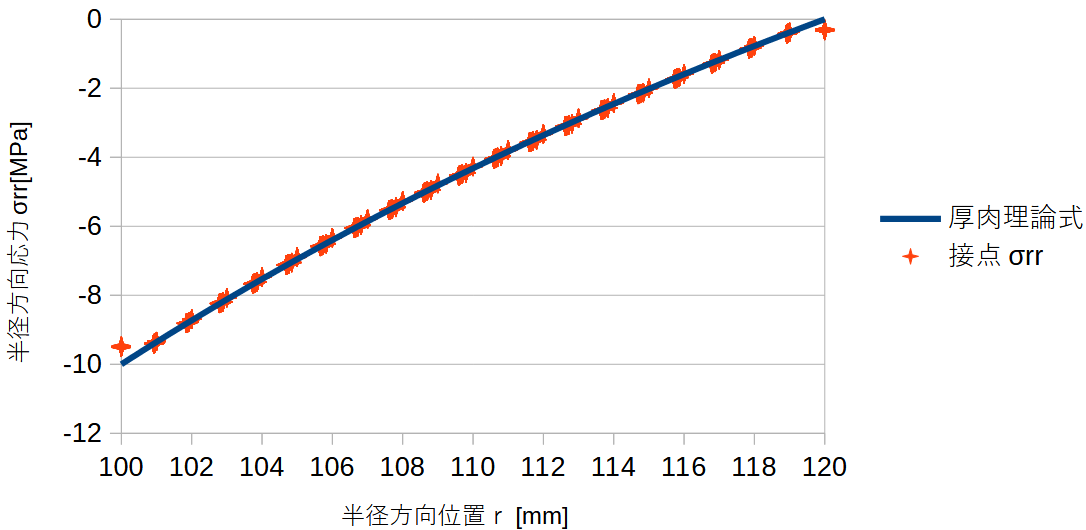
\includegraphics[width=\columnwidth]{work/images/results01.png}
     \caption{半径方向応力
       \begin{math}
         σ_{rr}
       \end{math}
     }
     \label{fig:hidari}
  \end{minipage}
%
  \begin{minipage}{0.49\columnwidth}
     \centering
     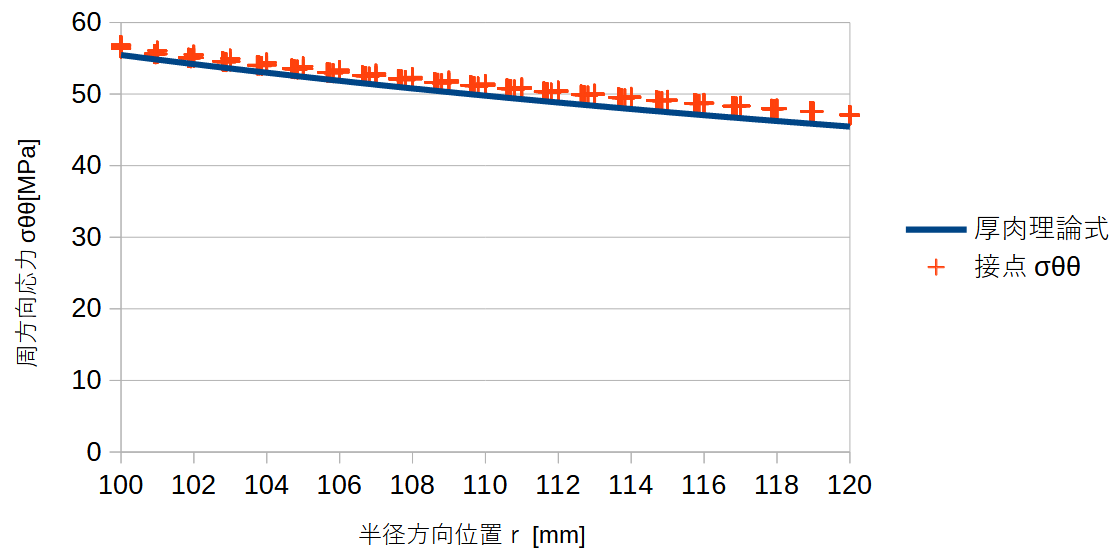
\includegraphics[width=\columnwidth]{work/images/results02.png}
     \caption{周方向応力
       \begin{math}
         σ_{\theta\theta}
       \end{math}
     }
     \label{fig:migi}
  \end{minipage}
\end{figure}

\end{frame}
